% \begin{savequote}[8cm]
% \textlatin{Cor animalium, fundamentum e\longs t vitæ, princeps omnium, Microco\longs mi Sol, a quo omnis vegetatio dependet, vigor omnis \& robur emanat.}

% The heart of animals is the foundation of their life, the sovereign of everything within them, the sun of their microcosm, that upon which all growth depends, from which all power proceeds.
%   \qauthor{--- William Harvey \cite{harvey_exercitatio_1628}}
% \end{savequote}

\chapter{\label{app:misleadingexplanations}Reference Materials for Misleading Explanations of AI Outputs in Talent Identification}

\minitoc

\section{Tasks}\label{sec:tasks}
Rather than an evaluation of a machine (where a user might rate a model as being correct because it is consistent), we restrict our analysis to human-in-the-loop tasks (where, if a user disagrees with a machine, they might override it) to better simulate and assess the sense in which a human-in-the-loop is \emph{vulnerable} to being mislead by an explanation.

Furthermore, we recognize that in many cases, a user's confidence in their own judgement would crowd out any possible effect of the AI system (and any associated explanation), or the ambiguity about whether any ground truth exists at all may lead a user to hold steadfast in their opinions. Thus, we avoid domains like ``is this an image of a cat?'' where it is obvious to the human whether the image is one of a cat. Similarly, we avoid tasks without a clear ground truth such as ``is this language offensive?'' or ``is this a good work of art?''. (Philosophers continue to argue whether or not these questions have objective answers. Kant, for example, contended that, while they do not admit objective answers, subjects are nonetheless justified in making universal claims \cite{zangwill_aesthetic_2023}.)

\begin{figure*}[htbp]
    \hspace{\fill}
    \subfloat[\label{survey_table_adult}]{
        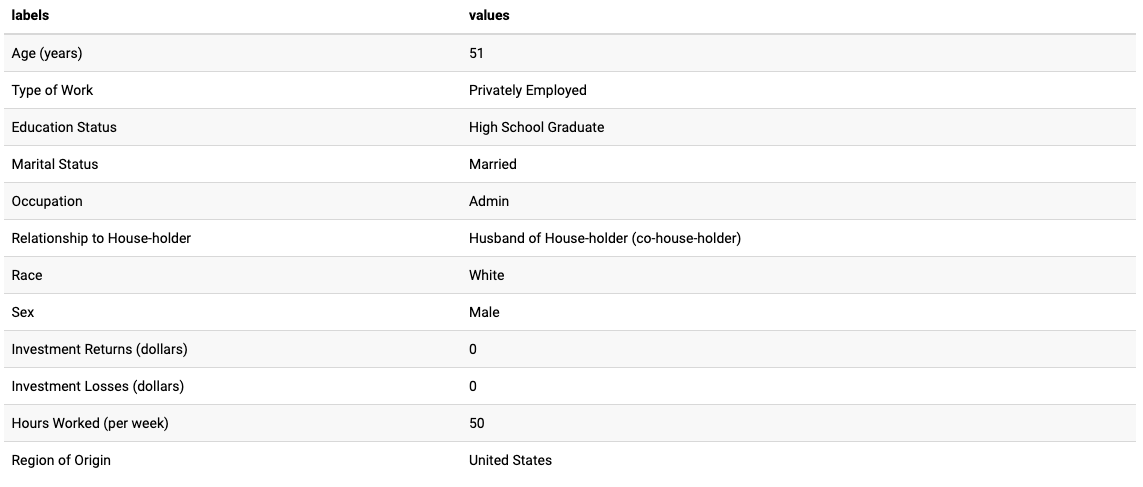
\includegraphics[clip, width=0.4\textwidth]{figures/misleading_explanations/survey_table_adult.png}}
    \hspace{\fill}
    \subfloat[\label{survey_table_credit} ]{
        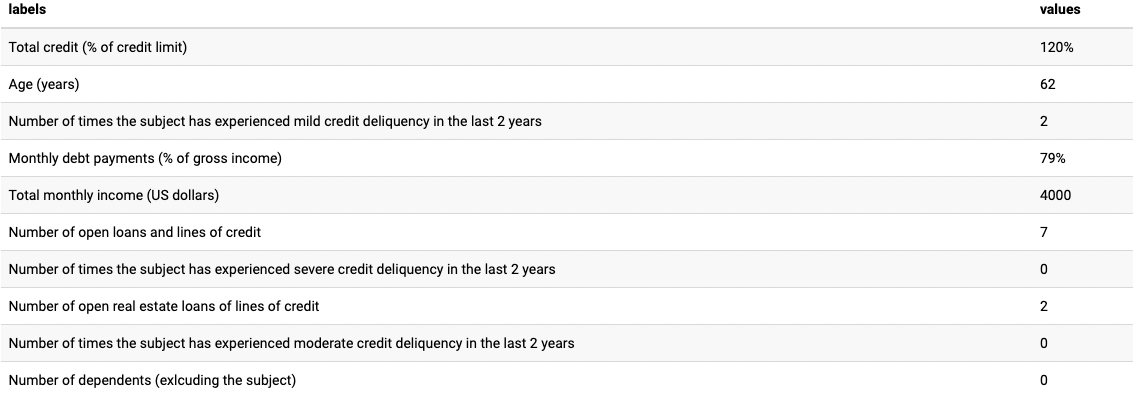
\includegraphics[clip, width=0.4\textwidth]{figures/misleading_explanations/survey_table_credit.png}}
    \hspace{\fill}
    \caption{Features from a Sample Case in (a) the Salary Estimation and (b) the Credit Prediction Tasks}
    \label{fig:survey_table}
\end{figure*}

\begin{figure*}[htbp]
    \hspace{\fill}
    \subfloat[\label{survey_pred_adult}]{
        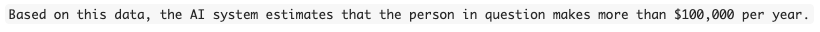
\includegraphics[clip, width=0.4\textwidth]{figures/misleading_explanations/survey_prediction_adult.png}}
    \hspace{\fill}
    \subfloat[\label{survey_pred_credit} ]{
        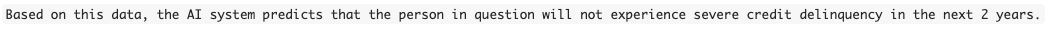
\includegraphics[clip, width=0.4\textwidth]{figures/misleading_explanations/survey_prediction_credit.png}}
    \hspace{\fill}
    \caption{Predictions from a Sample Case in (a) the Salary Estimation and (b) the Credit Prediction Tasks}
    \label{fig:survey_pred}
\end{figure*}

We choose two standard benchmark datasets: Adult and Give Me Some Credit \cite{kohavi_scaling_1996,GiveMeSomeCredit}. We choose these because such datasets are typically the grounds on which xAI methods are developed and critiqued. The Adult dataset specifically has been used as a benchmark in multiple xAI studies, including \textcite{weerts_case-based_2019}, \textcite{weerts_human-grounded_2019}, and \textcite{ribeiro_anchors_2018}. Various credit datasets, including Give Me Some Credit, are common as benchmarks in xAI studies like \textcite{bansal_does_2021}, \textcite{ustun_learning_nodate}, and \textcite{krishna_disagreement_2022}.

The dependent variable (to be estimated by the participant) of the Adult dataset is ``Does this person make more than \$50,000?''. However, we adjusted the amount due to inflation (this amount in 1994 is roughly \$100,000 today). Thus, we ask ``Does this person make more than \$100,000?''. The dependent variable of the Give Me Some Credit dataset is ``Will this person be at least 90 days delinquent on a credit payment in the next two years'', which we simplify to ``Will this person experience severe credit delinquency in the next two years'' (we also include a definition of ``severe credit delinquency'').

The participant has access to a table containing all data the model does in both cases; samples of these tables are shown in Figure \ref{fig:survey_table}. Figure \ref{fig:survey_pred} displays the initial estimate of the AI system for the very same samples, as they are shown to participants.

\section{Questions and Constructs}\label{sec:constructs}

We ask three questions both before and after explanation. In the Salary Estimation task, we ask ``How much money do you estimate this person makes?'', to which the possible responses are ``Less than \$100,000 per year'' and ``More than \$100,000 per year''. In the Credit Prediction task, we ask ``Do you predict that this person will experience severe credit delinquency?'', where the answers are ``Will not experience severe delinquency'' and ``Will experience severe delinquency''. In either case, this yields a binary $estimate$ variable. 

Then, we ask ``How confident are you in your estimation?'', which has a 20-point sliding scale of possible responses. This yields the $confidence$ (confidence) variable with a value between $1$ and $20$. 

Finally, we ask ``How much do you trust the AI system's estimation?'', which has a 20-point sliding scale of possible responses. This yields the attitudinal trust variable, $trust_{attitude}$, also with a value between $1$ and $20$. 

\begin{figure*}[htbp]
    \centering
    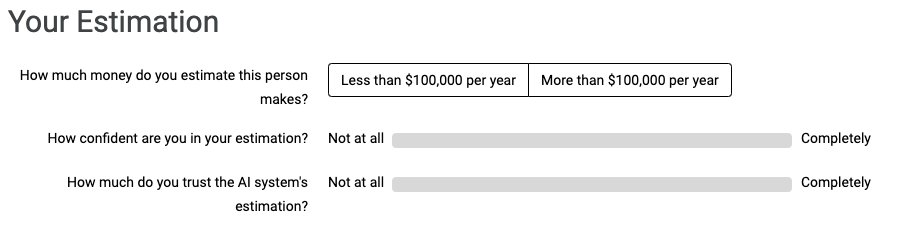
\includegraphics[width=0.8\textwidth]{figures/misleading_explanations/survey_question_adult.png}
    \caption{Three Questions Asked Twice per Case (Salary Estimation)}
    \label{fig:survey_question_adult}
\end{figure*}

\begin{figure*}[htbp]
    \centering
    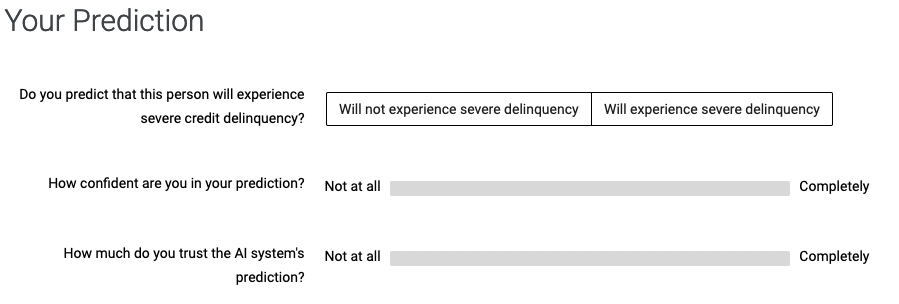
\includegraphics[width=0.8\textwidth]{figures/misleading_explanations/survey_question_credit.png}
    \caption{Three Questions Asked Twice per Case (Credit Prediction)}
    \label{fig:survey_question-credit}
\end{figure*}

These three questions are asked twice; once before the participant sees one of the three experimental conditions (SHAP, Anchors, and Confidence), and once again after. We index the `before' case as $before$ and the `after' case as $after$. 

Thus, we collect six variables from participants per case: $estimate^{before}$, $confidence^{before}$, $trust_{attitude}^{before}$, $estimate^{after}$, $confidence^{after}$, $trust_{attitude}^{after}$. The presentation of the three questions is shown in Figures \ref{fig:survey_question_adult} and \ref{fig:survey_question_credit}.

We also collect two additional variables per case: $answer$ and $recommendation$. In each case, $answer$ is the correct output for the case (as in our test output data), and $recommendation$ is the machine's recommendation of what the user should estimate for that case. 

We can now define some constructed variables for use in our analysis. First, we define a $agreement$ to be whether the user's estimate is in agreement with the machine's recommendation in Equation \ref{eq:trimp_agreement}. 

\begin{equation}
    agreement^x := estimate^x == recommendation
    \label{eq:trimp_agreement}
\end{equation}

We now define a variable $trust_{behaviour}$ in Equation \ref{eq:trimp}, which is a combination of the $estimate$, $confidence$, and $agreement$ variables to yield a $40$-point scale of behavioural trust. Here, $-19$ is absolute confidence that the system is wrong and $20$ is absolute confidence that the system is right. Let:

\begin{equation}
    trust_{behaviour}^x := \left\{
        \begin{array}{ll}
            confidence^x & \quad agreement^x\\
            1 - confidence^x & \quad otherwise
        \end{array}
    \right.
    \label{eq:trimp}
\end{equation}

In order to reason about the change in a variable due to the explanation, we define `$\Delta$' constructs as the difference between after- and before-explanation for each variable, as seen in Equation \ref{eq:deltas}.

\begin{equation}
    \Delta x := x^{after} - x^{before}
    \label{eq:deltas}
\end{equation}

Informally, $\Delta trust_{attitude}$ is the effect of the explanation on the participant's attitudinal trust in the AI determination. Formally, $\Delta trust_{attitude} := trust_{attitude}^{after} - trust_{attitude}^{before}$. E.g., suppose a participant sees a determination they believe to be incorrect in the absence of an explanation, they might express distrust in that system and rate their trust low (say $3$); suppose further that, the explanation provided is persuasive, and the participant rates their trust high (say $19$) after reading it; the $\Delta trust_{attitude}$ for this case would be $19 - 3 = 16$.

\section{Models}\label{sec:models}
In this study, we rely on three different models. We use a random forest classifier as our base model. We use a SHAP explainer to produce one of our explanatory conditions, and a Scoped Anchors explainer to produce another (our final explanatory condition is produced natively by the random forest). 

We opt for a random forest model as they are still ubiquitous in the field of AI, and the Adult and Give Me Some Credit datasets lack the kind of feature richness required to noticeably benefit from more sophisticated model architectures \cite{Grinsztajn_Oyallon_Varoquaux_2022}. The random forest classifiers classify points in each data set into either of the two outcome conditions. Our random forest classifier achieves 86\% test accuracy on the Adult dataset and 93\% test accuracy on the Give Me Some Credit dataset.

\begin{figure*}[htbp]
    \hspace{\fill}
    \subfloat[\label{survey_shap_adult}]{
        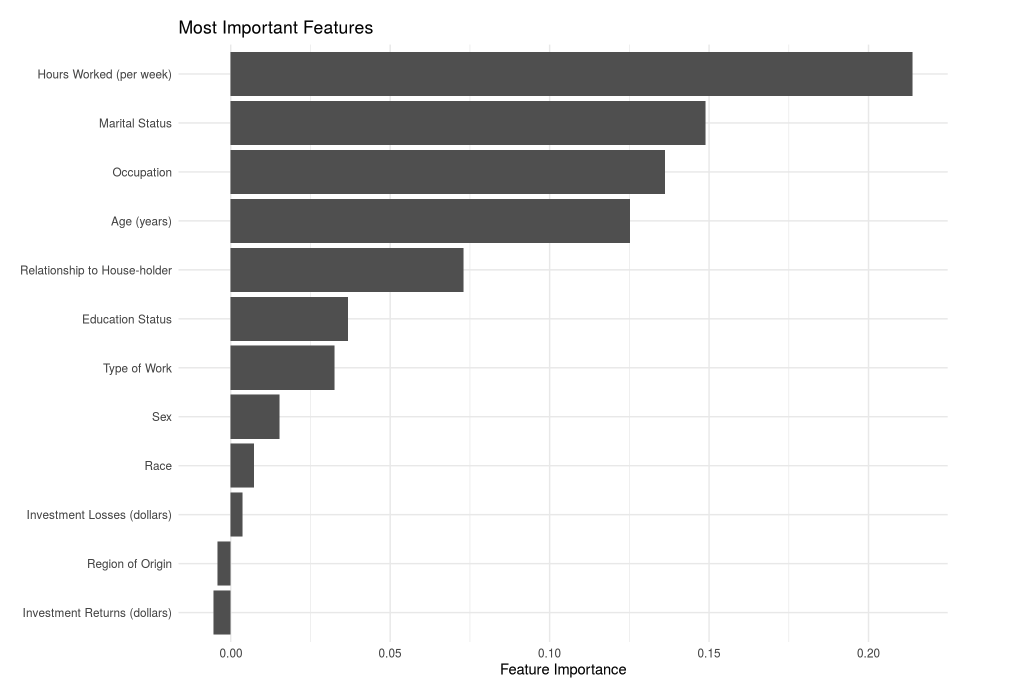
\includegraphics[clip, width=0.4\textwidth]{figures/misleading_explanations/survey_shap_adult.png}}
    \hspace{\fill}
    \subfloat[\label{survey_shap_credit} ]{
        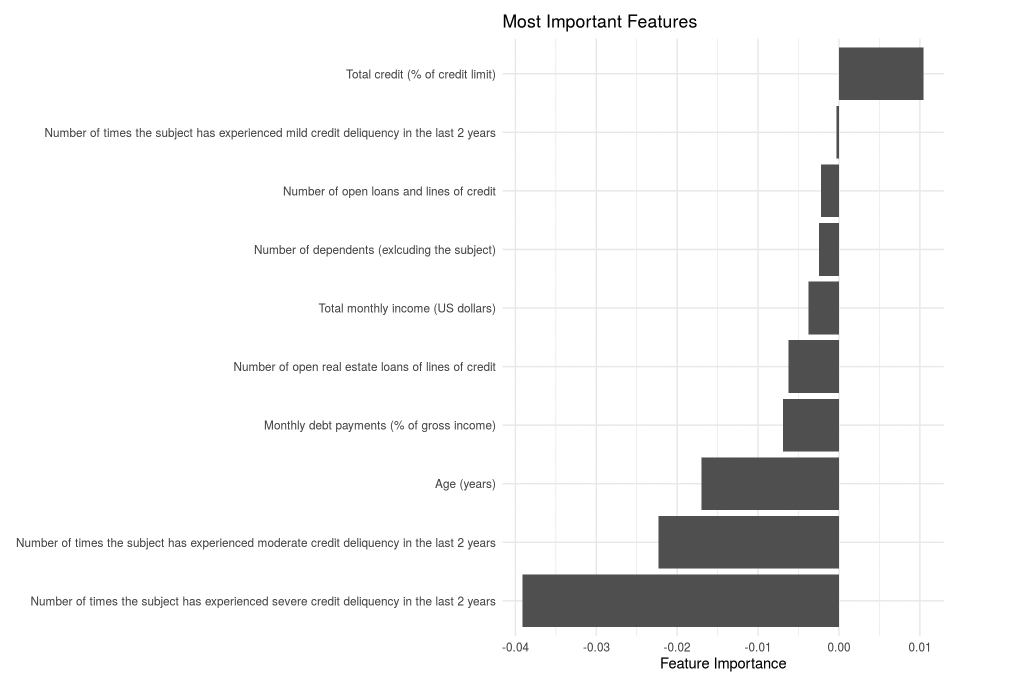
\includegraphics[clip, width=0.4\textwidth]{figures/misleading_explanations/survey_shap_credit.png}}
    \hspace{\fill}
    \caption{Sample SHAP Explanations in (a) the Salary Estimation and (b) the Credit Prediction Tasks}
    \label{fig:survey_shap}
\end{figure*}

\begin{figure*}[htbp]
    \hspace{\fill}
    \subfloat[\label{survey_anchor_adult}]{
        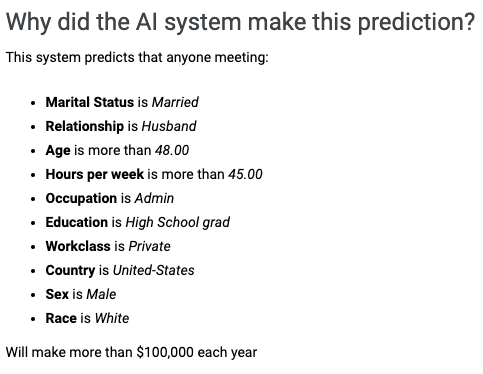
\includegraphics[clip, width=0.4\textwidth]{figures/misleading_explanations/survey_anchor_adult.png}}
    \hspace{\fill}
    \subfloat[\label{survey_anchor_credit} ]{
        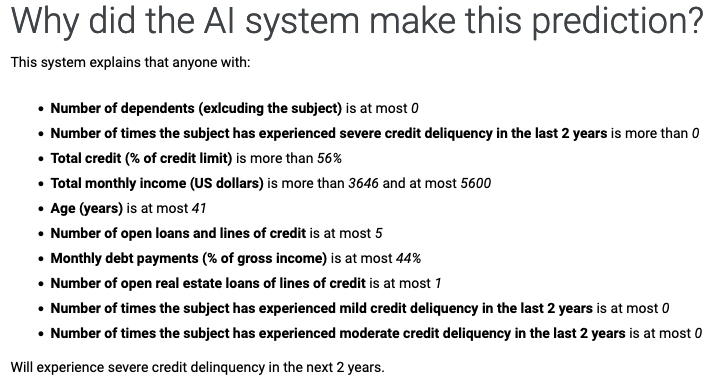
\includegraphics[clip, width=0.4\textwidth]{figures/misleading_explanations/survey_anchor_credit.png}}
    \hspace{\fill}
    \caption{Sample Anchors Explanations in (a) the Salary Estimation and (b) the Credit Prediction Tasks}
    \label{fig:survey_anchor}
\end{figure*}

\begin{figure*}[htbp]
    \hspace{\fill}
    \subfloat[\label{survey_confidence_adult}]{
        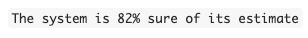
\includegraphics[clip, width=0.4\textwidth]{figures/misleading_explanations/survey_confidence_adult.png}}
    \hspace{\fill}
    \subfloat[\label{survey_confidence_credit} ]{
        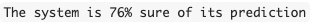
\includegraphics[clip, width=0.4\textwidth]{figures/misleading_explanations/survey_confidence_credit.png}}
    \hspace{\fill}
    \caption{Sample Confidence Explanations in (a) the Salary Estimation and (b) the Credit Prediction Tasks}
    \label{fig:survey_confidence}
\end{figure*}

Our three explanatory conditions are: SHAP, Anchors, and Confidence. SHAP explanations show participants a plot of feature importances, where the presented importances are the Shapley Values calculated for each feature. In the Anchors explanations, participants are shown rules that nearly guarantee that other cases following these rules will have the same estimate. In the Confidence condition, participants are shown the model's confidence in its estimate (based on the average output of all decision trees in the random forest model). We expect that providing any of these three explanations will generate an increase in trust even when the AI system is incorrect.

We select these three conditions carefully. We wish to test the popular feature importance explanation methods, of which SHapley-based Additive exPlanations, or SHAP (the `SHAP' condition), is a prominent example \cite{lundberg_unified_2017}. These explanations weight the importances of different features in a particular prediction. They are are often used to highlight aspects of the model to users and have been criticised in \textcite{kumar_problems_2020} for failing to follow norms of explanations drawn from philosophy, psychology, and cognitive science, making them bad candidates for explanation to end users. We also test the Scoped Anchors explanation algorithm (the `Anchors' condition) \cite{ribeiro_anchors_2018}. These explanations justify individual model predictions following human-centred norms by providing rules that bound model behaviour. \textcite{bansal_does_2021} and \textcite{jacobs_how_2021} both note that this styles of explanation raises user trust in a model. Finally, we also test the provision of the model's own confidence in its estimate (the `Confidence' condition). While confidence statistics are not generally regarded as an xAI method, they serve a similar function in that they indicate to the user something about the model's operation which allows evaluation of the model on those grounds.

We fine-tuned the visual design of each condition with a pilot study using the Adult dataset. In the pilot, we asked participants to indicate which of a range of visualisations is the most intuitive, and asked various questions to test their comprehension. For the SHAP condition, we found that a bar plot plotting feature importances, a format used for all feature importance methods across the field, appeared to be considered more intuitive \cite{weerts_human-grounded_2019}. As both models have relatively few features, we opted to show all features. For the Anchors condition, we found that a verbal explanation of the Anchors, mimicking formats used by popular social media platforms, was considered the most intuitive \cite{ribeiro_anchors_2018}. The formats used in the study itself can be seen in Figures \ref{fig:survey_shap}, \ref{fig:survey_anchor}, and \ref{fig:survey_confidence}.

\section{The Study}\label{sec:study}
We collected data in surveys designed and hosted on Formr.\footnote{www.formr.org} The participants were recruited via Prolific Academic's standard sampling method restricted to the United States (to match the origin of both datasets).\footnote{www.prolific.co}

Participants completed the study 6 times with 6 cases drawn from a pool of 39, where the AI system is correct on 20 out of the 39. To avoid learned effects related to the accuracy of either the model or the sample pool, participants were not told the machine accuracy or the distribution of the case pool. No participants were permitted to take part in both studies.